\documentclass[12pt]{article}
\usepackage[margin=1in]{geometry}
\usepackage{amsmath,amsthm,amssymb,epigraph,etoolbox,mathtools,setspace,enumitem} 
\usepackage{tikz}
\usepackage[makeroom]{cancel} 
\usepackage[linguistics]{forest}
\usetikzlibrary{patterns}
\newcommand{\N}{\mathbb{N}}
\newcommand{\Z}{\mathbb{Z}}
\newcommand{\R}{\mathbb{R}}
\newcommand{\Q}{\mathbb{Q}}

\def\rectangle{(-3,-3) rectangle(5,3)}
\def\firstcircle{(0,0) circle(2)}
\def\secondcircle{(2,0) circle(2)}

\newenvironment{theorem}[2][Theorem]{\begin{trivlist}
		\item[\hskip \labelsep {\bfseries #1}\hskip \labelsep {\bfseries #2.}]}{\end{trivlist}}
\newenvironment{lemma}[2][Lemma]{\begin{trivlist}
		\item[\hskip \labelsep {\bfseries #1}\hskip \labelsep {\bfseries #2.}]}{\end{trivlist}}
\newenvironment{exercise}[2][Exercise]{\begin{trivlist}
		\item[\hskip \labelsep {\bfseries #1}\hskip \labelsep {\bfseries #2.}]}{\end{trivlist}}
\newenvironment{problem}[2][Problem]{\begin{trivlist}
		\item[\hskip \labelsep {\bfseries #1}\hskip \labelsep {\bfseries #2.}]}{\end{trivlist}}
\newenvironment{question}[2][Question]{\begin{trivlist}
		\item[\hskip \labelsep {\bfseries #1}\hskip \labelsep {\bfseries #2.}]}{\end{trivlist}}
\newenvironment{corollary}[2][Corollary]{\begin{trivlist}
		\item[\hskip \labelsep {\bfseries #1}\hskip \labelsep {\bfseries #2.}]}{\end{trivlist}}
\newenvironment{solution}[2][Solution]{\begin{trivlist}
		\item[\hskip \labelsep {\bfseries #1}\hskip \labelsep {\bfseries #2.}]}{\end{trivlist}}

\setlength\epigraphwidth{8cm}
\setlength\epigraphrule{0pt}

\makeatletter
\patchcmd{\epigraph}{\@epitext{#1}}{\itshape\@epitext{#1}}{}{}
\makeatother


\begin{document}
	
	\title{Week 7}
	\author{Juan Patricio Carrizales Torres \\
		Section 3: Set Operations}
	\date{September 02, 2021}
	\maketitle
	
	\begin{problem}{23}
		Give examples of two sets $A$ and $B$ such that $|A-B|=|A\cap B|=|B-A|=3$. Draw the accompanying Venn diagram.
		\begin{solution}{} 
			Because $|A-B|=3$, it follows that there must be 3 elements in $A$ which do not belong to $B$. On the other hand, $|B-A|=3$ implies that there are 3 elements in $B$ such that they do not belong to $A$. Finally, there must be 3 elements that belong to both $A$ and $B$ since $|A\cap B|=3$.
			Two sets $A$ and $B$ that fulfill this conditions are\\
			$A=\{1,2,3,4,5,6\}$\\
			$B=\{4,5,6,7,8,9\}$\\
			The set $A-B=\{1,2,3\}$, 
			$A\cap B= \{4,5,6\}$, and 
			$B-A= \{7,8,9\}$.
			Therefore, $|A-B|=|A\cap B|=|B-A|=3$.
			\begin{center}
				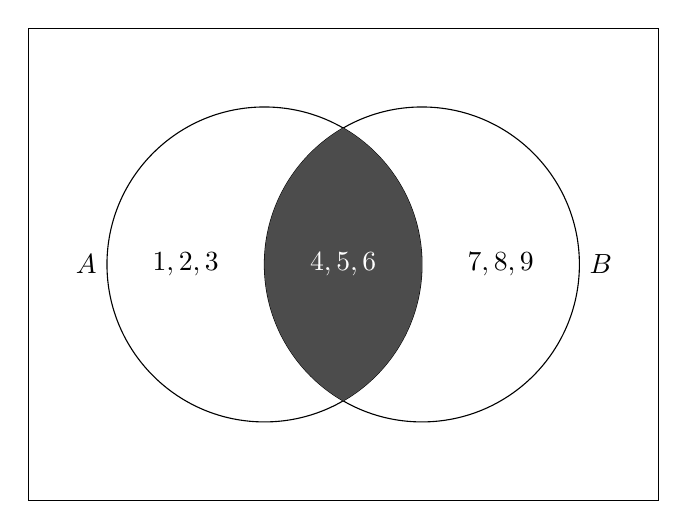
\begin{tikzpicture}
					\draw (-3,-3) rectangle (5,3);
					%A-B
					%\filldraw[pattern=dots] (0,0) circle(2);
					\node [draw, circle, minimum size= 4cm, label = {180:$A$}] (A) at (0,0){};
					%B-a
					\node [draw, circle, minimum size= 4cm, label = {0:$B$}] (A) at (2,0){};
					
					\scope %A\capB
					\clip (0,0) circle(2cm);
					\fill[black!70] (2,0) circle(2cm);
					\endscope
					
					%labels
					\node at (-1,0) {$1,2,3$};
					\node [text=white]at (1,0) {$4,5,6$};
					\node at (3,0) {$7,8,9$};
				\end{tikzpicture}
			\end{center}
		\end{solution}
	\end{problem}
	
	\begin{problem}{24}
		Give examples of three sets $A$, $B$ and $C$ such that $B \neq C$ but $B-A=C-A$
		\begin{solution}{}
			Since $B-A=C-A$, it follows that the elements of $C$ and $B$ that do not belong to $A$ must be the same. Also, $B\cap A \neq C\cap A$ so that $B\neq C$. 
			Let \\ $A=\{3\}$\\ $B=\{3,5\}$\\$C=\{5\}$\\
			Then,$B-A=\{5\}$, and $C-A=\{5\}$. Thus, $B\neq C$ but $B-A=C-A$ 
		\end{solution}
	\end{problem}

	\begin{problem}{26}
		Let $U$ be a universal set and let $A$ and $B$ be two subsets of $U$. Draw a Venn diagram for each of the following sets.\\
		(a) $\overline{A\cup B}$
		\begin{solution}{a}
			$\overline{A\cup B} = \{x:x\in U \text{ and } x\notin A\cup B\}$.\\ Note that $A\cup B= \{x:x\in A \text{ or } x\in B\}$
			\begin{center}
			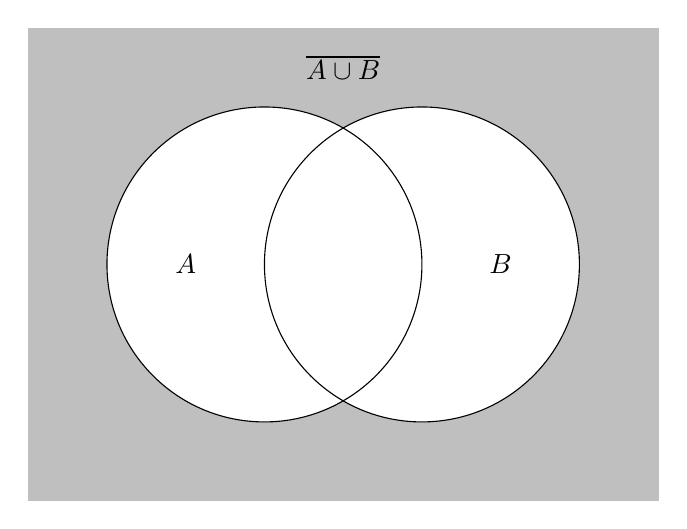
\begin{tikzpicture}
				\filldraw [gray!50] \rectangle;
				\fill [white] \firstcircle;
				\fill [white] \secondcircle;
				
				%drawing outlines of the circles
				\draw \firstcircle node at (-1,0){$A$};
				\draw \secondcircle node at (3,0){$B$};
				
				\node at (1,2.5){$\overline{A\cup B}$};
			\end{tikzpicture}
			\end{center}
		\end{solution}
		(b) $\overline{A}\cap\overline{B}$
		\begin{solution}{b}
			$\overline{A}\cap\overline{B}= \{x:x\in \overline{A} \text{ and } x\in \overline{B}\}$\\
			Note that $\overline{A} = \{x:x\in U \text{ and } x\notin A\}$ and $\overline{B} = \{x:x\in U \text{ and } x\notin B\}$. Therefore,  $\overline{A}\cap\overline{B}$ is the set of all $x\in U$ such that they don't belong to $A\cup B$.
			\begin{center}
				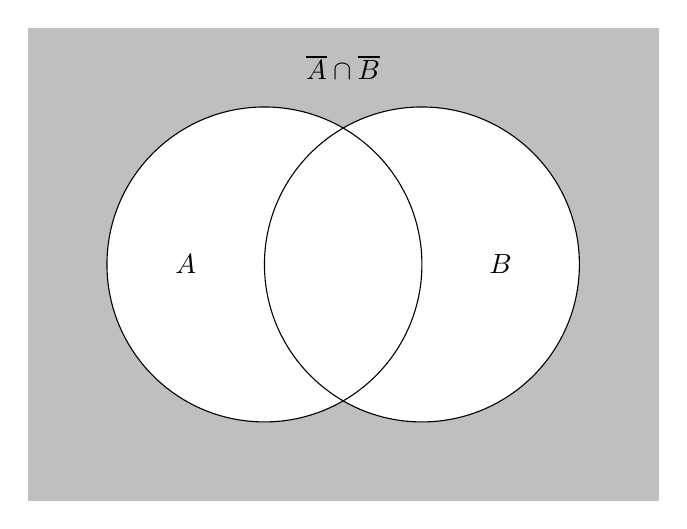
\begin{tikzpicture}
					\filldraw [gray!50] \rectangle;
					\fill [white] \firstcircle;
					\fill [white] \secondcircle;
					
					%drawing outlines of the circles
					\draw \firstcircle node at (-1,0){$A$};
					\draw \secondcircle node at (3,0){$B$};
					
					\node at (1,2.5){$\overline{A}\cap \overline{B}$};
				\end{tikzpicture}
			\end{center}
		\end{solution}
		It can be seen that, $\overline{A\cup B}=\overline{A}\cap \overline{B}$.\\
		(c) $\overline{A\cap B}$ 
		\begin{solution}{c}
			$\overline{A\cap B} = \{x:x\in U \text{ and } x\notin A\cap B\}$. 
				\begin{center}
				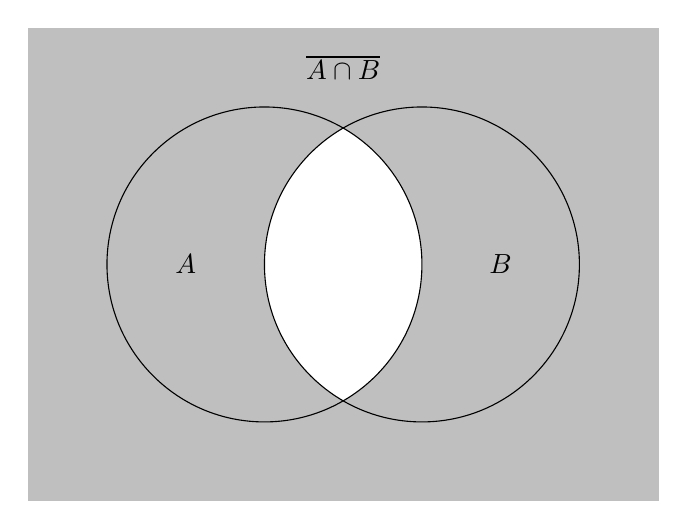
\begin{tikzpicture}
					\filldraw [gray!50] \rectangle;
					
					\scope
					\clip  \firstcircle;
					\fill [white] \secondcircle;
					\endscope
					
					%drawing outlines of the circles
					\draw \firstcircle node at (-1,0){$A$};
					\draw \secondcircle node at (3,0){$B$};
					
					\node at (1,2.5){$\overline{A\cap B}$};
				\end{tikzpicture}
			\end{center}
		\end{solution}
	(d) $\overline{A}\cup \overline{B}$
	\begin{solution}{d}
		$\overline{A}\cup \overline{B}=\{x:x\in \overline{A} \text{ or } x\in \overline{B} \}$.\\
		Thus, the set $\overline{A}\cup \overline{B}$ contains all $x\in U$ that don't belong to $A$ or don't belong to $B$.
			\begin{center}
			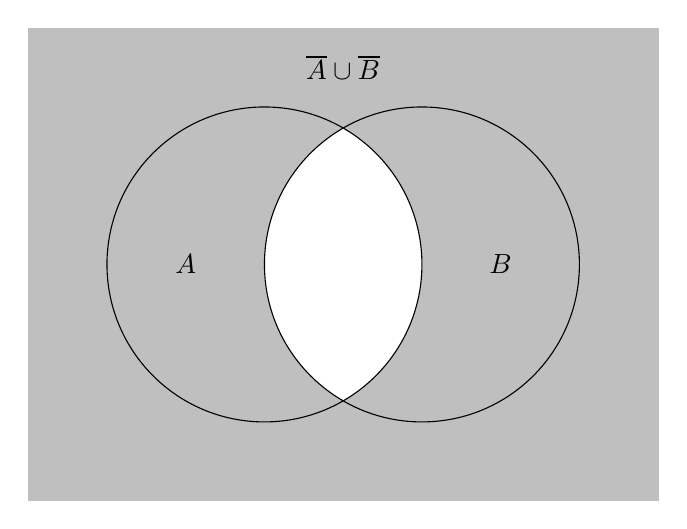
\begin{tikzpicture}
				\filldraw [gray!50] \rectangle;
				
				\scope
				\clip  \firstcircle;
				\fill [white] \secondcircle;
				\endscope
				
				%drawing outlines of the circles
				\draw \firstcircle node at (-1,0){$A$};
				\draw \secondcircle node at (3,0){$B$};
				
				\node at (1,2.5){$\overline{A}\cup \overline{B}$};
			\end{tikzpicture}
		\end{center}
	It can be seen that, $\overline{A\cap B}=\overline{A}\cup \overline{B}$.
	\end{solution}
	\end{problem}

\begin{problem}{32}
	Give an example of four different subsets $A$, $B$, $C$ and $D$ of $\{1,2,3,4\}$ such that all intersections of two subsets are different.
	\begin{solution}{}
		The subset $A$ can be the set $\{1,2,3,4\}$ since every set is a subset of itself. Each subset $B$, $C$ and $D$  takes one different number from $A$ so that their intersections with $A$ differ and they are not equal. Then, both $B$ and $C$ can take the number that only $A$ contains, now they got an intersection. Lastly, $D$ takes one element $x$ of either $B$ or $C$ such that $x\notin B\cap C$.\\ Let
		$A=\{1,2,3,4\}$\\
		$B=\{1,4\}$\\
		$C=\{2,4\}$\\
		$D=\{3,1\}$\\
		Then, $A\cap B= \{1,4\}$, $A\cap C= \{2,4\}$, $A\cap D=\{1,3\}$, $B\cap C=\{4\}$, $B\cap D= \{1\}$, $C\cap D= \emptyset$
	\end{solution}
\end{problem}
\begin{problem}{33}
	Give an example of two nonempty sets $A$ and $B$ such that $\{A\cup B, A\cap B, A-B, B-A\}$ is the power set of some set.
	\begin{solution}{}
		Let $D$ be a set and $\mathcal{P}(D)=\{A\cup B, A\cap B, A-B, B-A\}$ be its power set. Because  $|\mathcal{P}(D)|=2^{|D|}=4$, it follows that $|D|=2$. Therefore, $D=\{n,m\}$ for some elements $n,m$ and  $\mathcal{P}(D)=\{\emptyset, \{n\}, \{m\}, \{n,m\}\}$.
		The cardinality $|A\cup B|$ must be greater than that of the other sets $A\cap B$, $A-B$ and $B-A$ since they are subsets of $A\cup B$. Thus, $A\cup B= \{n,m\} = D$. It is possible that $A=\{n\}$ and $B=\{m\}$.\\
		Let,\\
		$A=\{1\}$\\
		$B=\{2\}$\\
		$D=\{1,2\}$\\
		Then, $\mathcal{P}(D)=\{\emptyset, \{1\},\{2\},\{1,2\}\}$ and $A\cup B = \{1,2\}$, $A-B=\{1\}$, $B-A=\{2\}$, $A\cap B= \emptyset$.
	\end{solution}
\end{problem}
\begin{problem}{34}
	Give an example of two subsets $A$ and $B$ of $\{1,2,3\}$ such that all of the following sets are different: $A\cup B$, $A\cup \overline{B}$, $\overline{A}\cup B$, $\overline{A}\cup \overline{B}$, $A\cap B$, $A\cap \overline{B}$, $\overline{A}\cap B$, $\overline{A}\cap \overline{B}$.
	\begin{solution}{}
	under construction
	\end{solution}
\end{problem}
\begin{problem}{35}
	Give examples of a universal set $U$ and sets $A$, $B$ and $C$ such that each of the following sets contains exactly one element: $A\cap B\cap C, (A\cap B)-C, (A\cap C)-B, (B\cap C)-A, A-(B\cup C), B-(A\cup C), C- (A \cup B), \overline{A\cup B\cup C}$. Draw the accompanying Venn diagram.
	\begin{solution}{}
		Using a Venn Diagram will facilitate the process of coming up with a solution for this problem since each of the sets that must contain one element represent a section of the following Venn diagram and they don't intersect each other.
		\begin{center}
			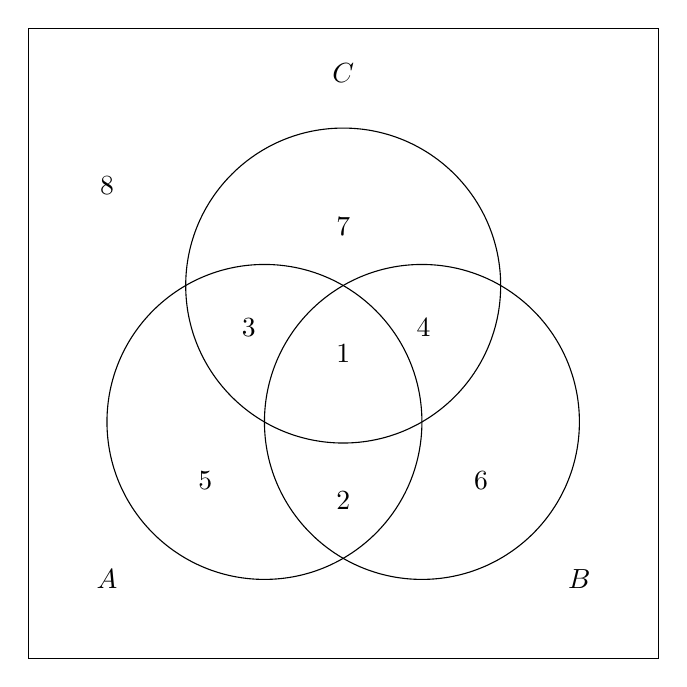
\begin{tikzpicture}
				\draw (-3,-3) rectangle(5,5);
				
				%drawing outlines of the circles
				\draw \firstcircle node at (-0.75,-0.75){$5$};
				\draw \secondcircle node at (2.75,-0.75){$6$};
				\draw (1,1.732) circle(2) node at (1,1.732+0.75){$7$};
				 
				\node at (-2,-2){$A$};
				\node at (4,-2){$B$};
				\node at (1, 1.732 +2.7){$C$};
				\node at (-2,3){$8$};
				\node at (-0.2,1.2){$3$};
				\node at (2.02, 1.2){$4$};
				\node at (1, -1){$2$};
				\node at (1,1.732/2){$1$};
			\end{tikzpicture}
	\end{center}
		Let, $U=\{1,2,3,4,5,6,7,8\}$\\
		$A=\{1,2,3,5\}$\\
		$B=\{1,2,4,6\}$\\
		$C=\{1,3,4,7\}$\\
		Then, $A\cap B\cap C= \{1\}$, $(A\cap B)-C=\{2\}$, $(A\cap C)-B=\{3\}$, $(B\cap C)-A=\{4\}$, $A-(B\cup C)=\{5\}$, $B-(A\cup C)=\{6\}$, $C-(A\cup B)=\{7\}$, $\overline{A\cup B\cup C}=\{8\}$.
	\end{solution}
\end{problem}
\end{document}